\section{Evaluation}

\subsection{Experimental Setup}
\label{sec:setup}


\paragraph{Baselines.} We evaluate \roomie{} against two different state-of-the-art baselines: INFaaS and Usher. INFaaS performs accuracy scaling by scaling variants within the same worker to meet demand. Usher, on the other hand, groups compute-heavy models with memory-heavy models within a group. We have used different models from two family groups, namely classification and detection, to evaluate our solution and baselines. We consider that each incoming query is intended for a single inference model.

\paragraph{Deployment Infrastructure.} We conducted our experiments using two distinct deployment types: a cluster of Jetson Nanos and a cluster of larger \acrshort{gpu}s. The first consisted of $3\times$ machines equipped with $4\times$ Nvidia \textit{A100-SXM4-40GB (40 GiB)}. The second consisted of $12\times$ Nvidia Jetson AGX Xavier \acrshort{gpu}s. Each \acrshort{gpu} is assigned to a docker to form a server, making a total of 12 servers for each deployment. We also used $2\times$ HPE Proliant DL360 Gen10+ the client requesting the model and a controller responsible for serving requests to workers. The full specifications are presented in \Cref{tab:serve_config}.

\begin{table}
	\centering
	\begin{tabular}{p{2cm}p{3cm}p{3cm}}
		\toprule
		\textbf{Model}            & \textbf{CPU}                                & \textbf{\acrshort{gpu}}                                                 \\
		\toprule

		Nvidia Jetson AGX Xavier  & 1 CPU/node, 8 cores/CPU                     & Nvidia AGX Xavier, CC~\footnote{CC: Compute capability}: 7.2 \\

		\midrule

		HPE Proliant DL360 Gen10+ & x86\_64, 2.40GHz, 2 CPUs/node, 16 cores/CPU &                                                              \\

		\midrule

		Apollo 6500 Gen10+        & x86\_64, 1 CPU/node, 32 cores/CPU           & $4\times$ Nvidia A100-SXM4-40GB (40 GiB), CC: 8.0            \\

		\midrule

		DL360 Gen10+              & x86\_64, 2.60GHz, 2 CPUs/node, 32 cores/CPU &                                                              \\

		\bottomrule
	\end{tabular}
	\caption{Server configuration used for experiments.}
	\label{tab:serve_config}
\end{table}

\paragraph{Datasets.} We evaluated our system and baseline methods using both synthetic and real-world workloads. For the real workload, we adopt the Twitter trace 2020 dataset~\cite{twitterStreamTrace2020}, as it is particularly suitable for modeling inference services, as tweets are commonly subjected to~\acrfull{dnn} processing before publication~\cite{francisco2021infaas,ahmad2024proteus}. Since the trace is aggregated at a coarse temporal granularity of one second, we apply a Poisson process to model intra-second arrival times and use a Zipf distribution to distribute queries among models, in line with established methodology~\cite{francisco2021infaas,ahmad2024proteus}.
For synthetic workloads, we generated average request rates per second using a Gaussian process and applied the same Zipf-based model allocation. To ensure our evaluation captures a broad spectrum of inference behavior, we selected a diverse and representative set of~\acrshort{dnn} models. These include both high-performance classification architectures and widely adopted object detection frameworks, enabling us to rigorously assess system behavior under varied computational and latency profiles. The full list of models is summarized in~\Cref{tab:dnn-models}, reflecting the breadth and relevance of our evaluation design.

\begin{table}[h]
	\centering \caption{Categorization of \acrlong{dnn} Models Used in Evaluation} \label{tab:dnn-models}
	\begin{tabular}{p{4cm}p{6cm}}
		\hline
		\textbf{Category} & \textbf{Models}
		\\ \hline
		Classification Models &
		\texttt{vgg19},
		\texttt{alexnet},
		\texttt{maxvit\_t},
		\texttt{resnet152},
		\texttt{googlenet},
		\texttt{densenet201},
		\texttt{squeezenet1\_1},
		\texttt{mobilenet\_v3\_large},
		\texttt{shufflenet\_v2\_x2\_0},
		\texttt{inception\_v3},
		\texttt{wide\_resnet101\_2},
		\texttt{resnext101\_32x8d},
		\texttt{efficientnet\_v2\_l},
		\texttt{convnext\_large}
		\\ \hline
		Object Detection Models &
		\texttt{ssd300\_vgg16},
		\texttt{fcos\_resnet50\_fpn},
		\texttt{retinanet\_resnet50\_fpn\_v2},
		\texttt{fasterrcnn\_resnet50\_fpn\_v2},
		\texttt{ssdlite320\_mobilenet\_v3\_large}
		\\ \hline 
	\end{tabular}
\end{table}

\paragraph{Evaluation Metrics.} To evaluate the effectiveness of each \acrshort{dnn} deployment strategy, the assessment focused on four key performance indicators. Response time measured how quickly the models delivered results, which is a critical indicator of real-time performance. The processing rate indicated the percentage of requests successfully processed, highlighting the reliability of the system for different workloads. Throughput measured the number of requests processed in a given time frame, providing insight into overall capacity and scalability. Finally, \acrshort{gpu} utilization monitored the degree of hardware resource usage during model execution.


\subsection{Performance Evaluation of Cloud-Based \acrshort{gpu} Cluster Solutions}

To assess the effectiveness of our proposed deployment strategy, we conducted a comprehensive evaluation using a cloud-based \acrshort{gpu} cluster comprising 12$\times$ \acrshort{gpu}s and all~\acrshort{dnn} models detailed in~\Cref{tab:dnn-models}. The experiments were performed using two distinct datasets: real-world Twitter data and synthetically generated data. These synthetic workloads were constructed to mimic real-world traffic patterns while allowing precise manipulation of query rates. This enabled a more granular analysis of system behavior under stress. These datasets were used to simulate varying workload intensities, beginning with low traffic levels that all models could handle and gradually increasing until system saturation was observed.

\paragraph{Evaluation on Twitter dataset.}

\begin{figure}[h!]
	\centering
	\begin{subfigure}[b]{0.45\textwidth}
		\centering
		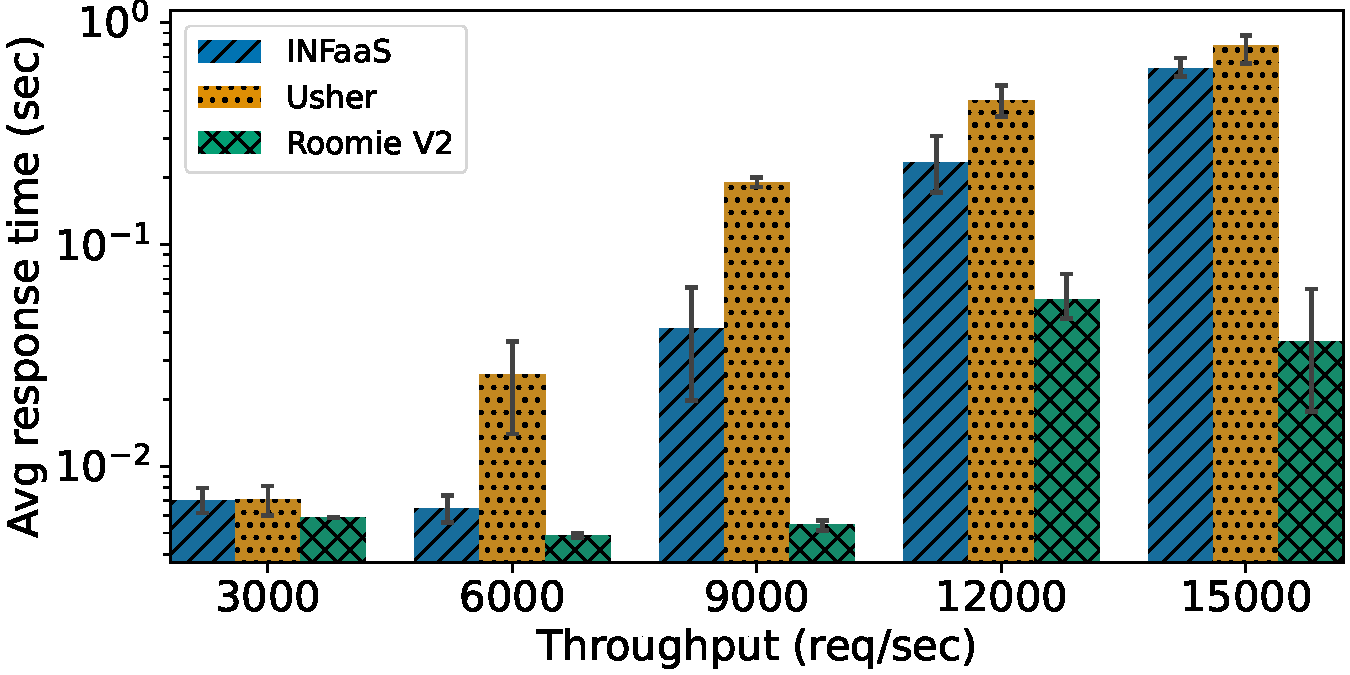
\includegraphics[width=\textwidth]{chapters/roomie/images/NvidiaA100/twitter-all-models/response_time.pdf}
		\subcaption{Response time.}
	\end{subfigure}
	\hfill
	\begin{subfigure}[b]{0.45\textwidth}
		\centering
		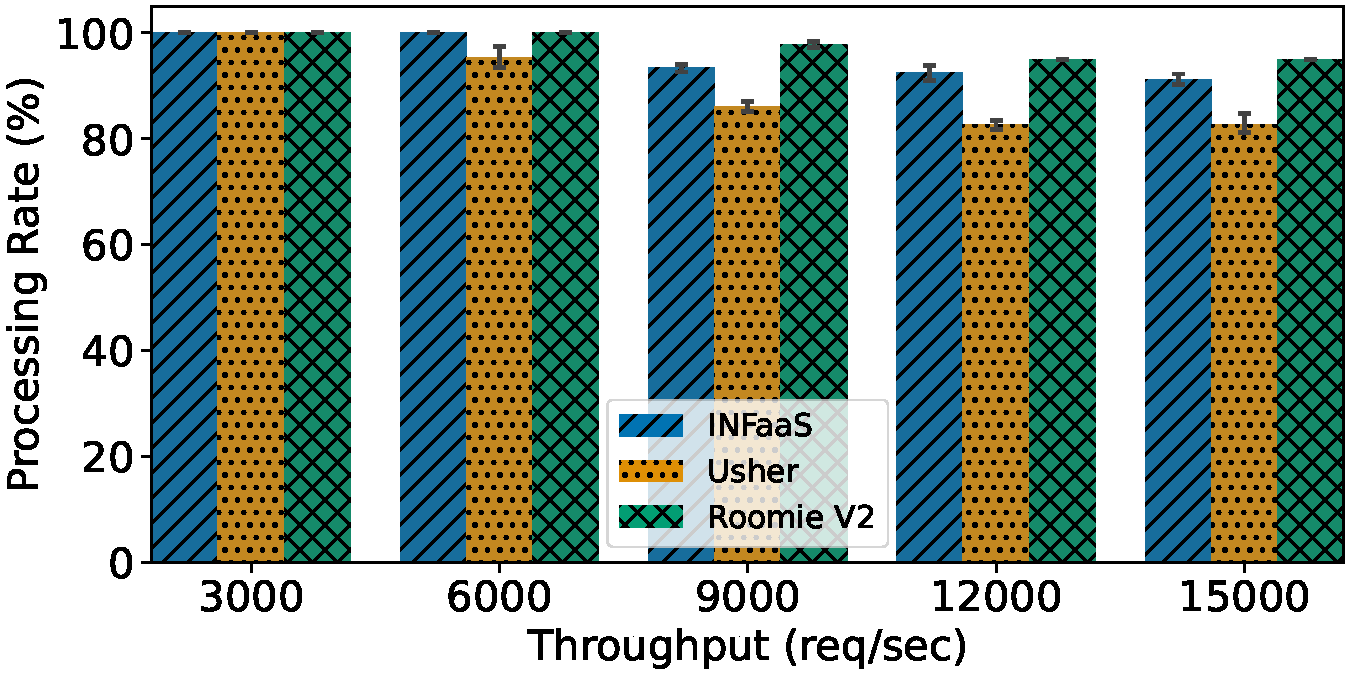
\includegraphics[width=\textwidth]{chapters/roomie/images/NvidiaA100/twitter-all-models/normalized.pdf}
		\subcaption{Processing rate.}
	\end{subfigure}
	
	\vspace{0.5cm} % Space between the rows
	
	\begin{subfigure}[b]{0.45\textwidth}
		\centering
		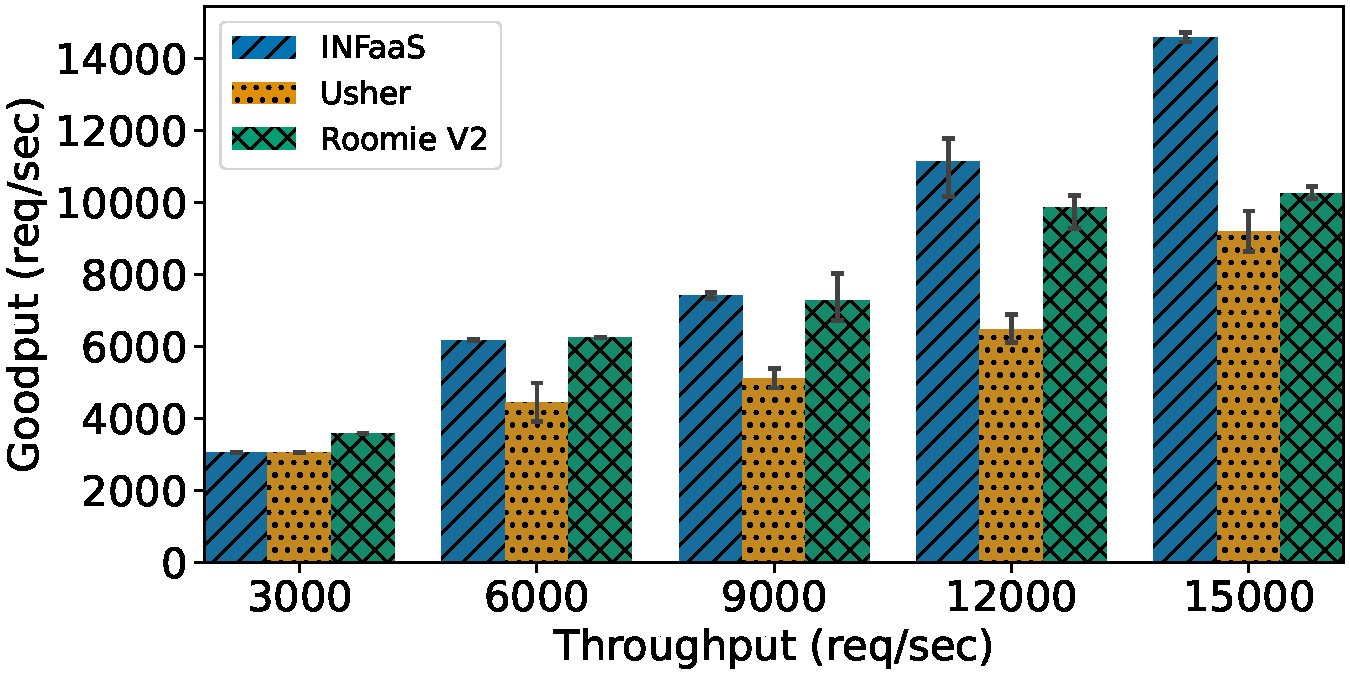
\includegraphics[width=\textwidth]{chapters/roomie/images/NvidiaA100/twitter-all-models/goodput.pdf}
		\subcaption{Goodput.}
	\end{subfigure}
	\hfill
	\begin{subfigure}[b]{0.45\textwidth}
		\centering
		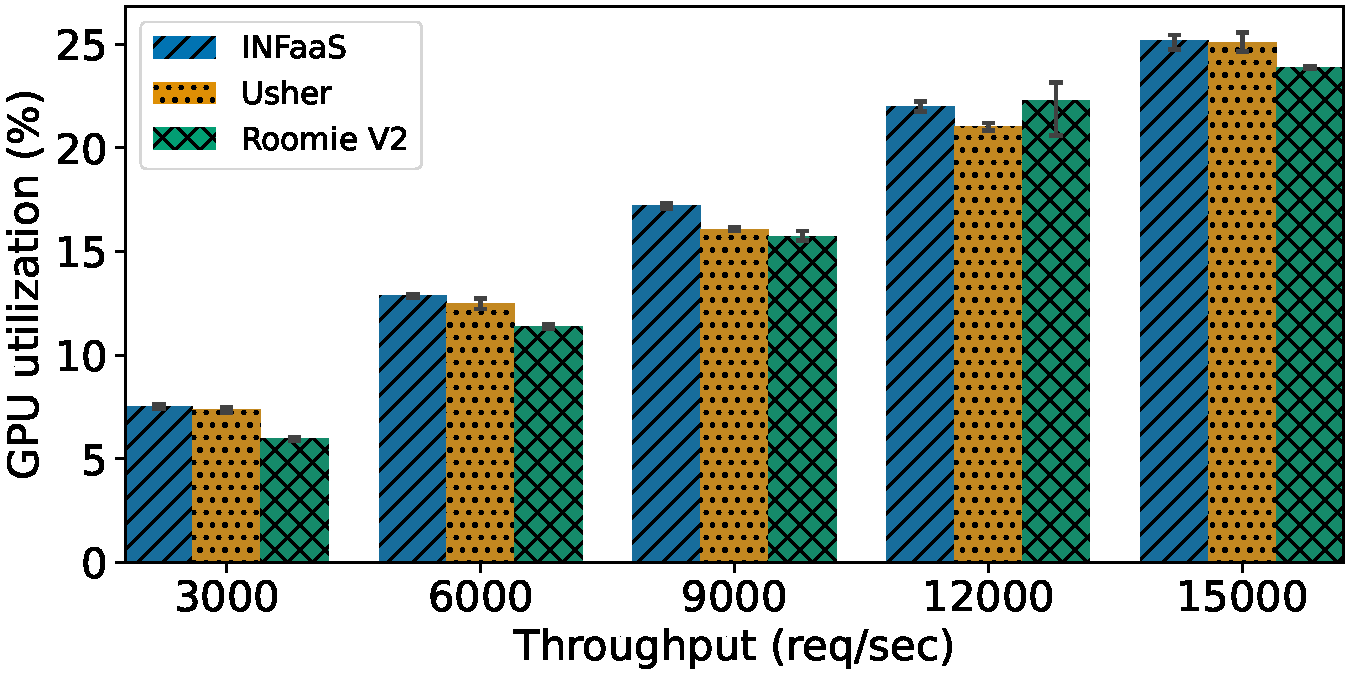
\includegraphics[width=\textwidth]{chapters/roomie/images/NvidiaA100/twitter-all-models/gpu_utilization.pdf}
		\subcaption{\acrshort{gpu} utilization}
	\end{subfigure}
	
	\caption{\roomie{} achieves up to 17$\times$ faster response times while delivering similar processing rates in a cloud-based evaluation using the Twitter dataset, outperforming INFaaS and Usher under high workload conditions.}
	\label{fig:NvidiaA100/twitter-all-models}
\end{figure}


\Cref{fig:NvidiaA100/twitter-all-models} shows the performance results obtained from the Twitter database. Under low workload conditions, all approaches showed comparable response times. However, as the workload increased, significant performance disparities emerged. Notably,~\roomie{} achieved response times up to 17× faster than rival solutions and maintained a processing rate above 97\%. In contrast, Usher's strategy of co-locating large models with lightweight models failed to deliver satisfactory performance under high load, resulting in increased latency and reduced goodput. INFaaS, which scales \acrshort{dnn}s on workers already hosting a copy, showed moderate goodput performance. However, this approach is agnostic to model interference, leading to latency increases of up to 17× and a decline in processing rate.

Interestingly, despite low \acrshort{gpu} utilization across all approaches, we observe a significant increase in response time as workload intensifies. This counterintuitive behavior can be attributed to the saturation of large models, which become unable to keep pace with incoming queries. As these models reach their computational limits, they begin to queue requests, leading to latency explosions—even though the \acrshort{gpu} itself remains underutilized. Additionally, interference between co-located models can further degrade responsiveness, compounding delays without a corresponding rise in \acrshort{gpu} activity. One potential mitigation strategy is to increase batch sizes, which can improve utilization by amortizing overhead across multiple queries. However, this approach introduces a trade-off: larger batches may inflate response times, making it unsuitable for latency-sensitive applications. These findings underscore the need for deployment strategies that go beyond raw utilization metrics and account for model saturation dynamics and cross-model interference.


\paragraph{Evaluation on synthetic dataset.}

\begin{figure}[h!]
	\centering
	\begin{subfigure}[b]{0.45\textwidth}
		\centering
		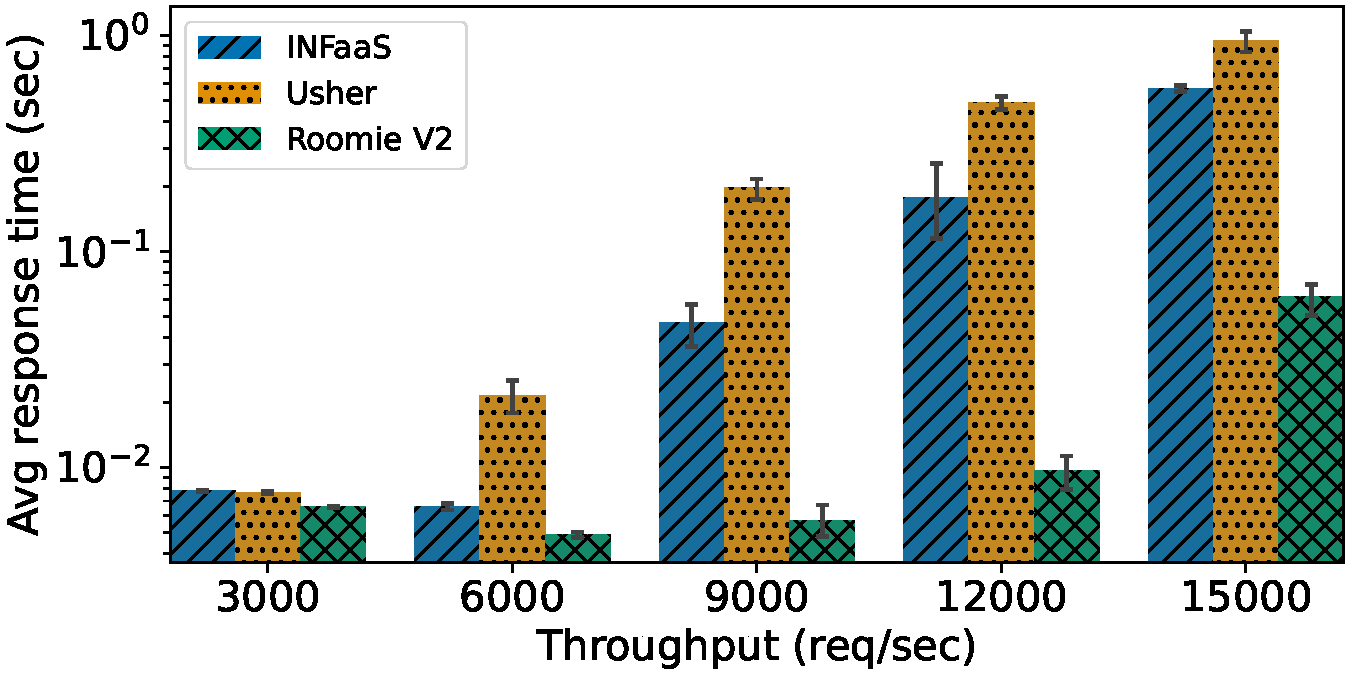
\includegraphics[width=\textwidth]{chapters/roomie/images/NvidiaA100/synthetic-all-models/response_time.pdf}
		\subcaption{Response time.}
		\label{fig:NvidiaA100/synthetic-all-models/response-time}
	\end{subfigure}
	\hfill
	\begin{subfigure}[b]{0.45\textwidth}
		\centering
		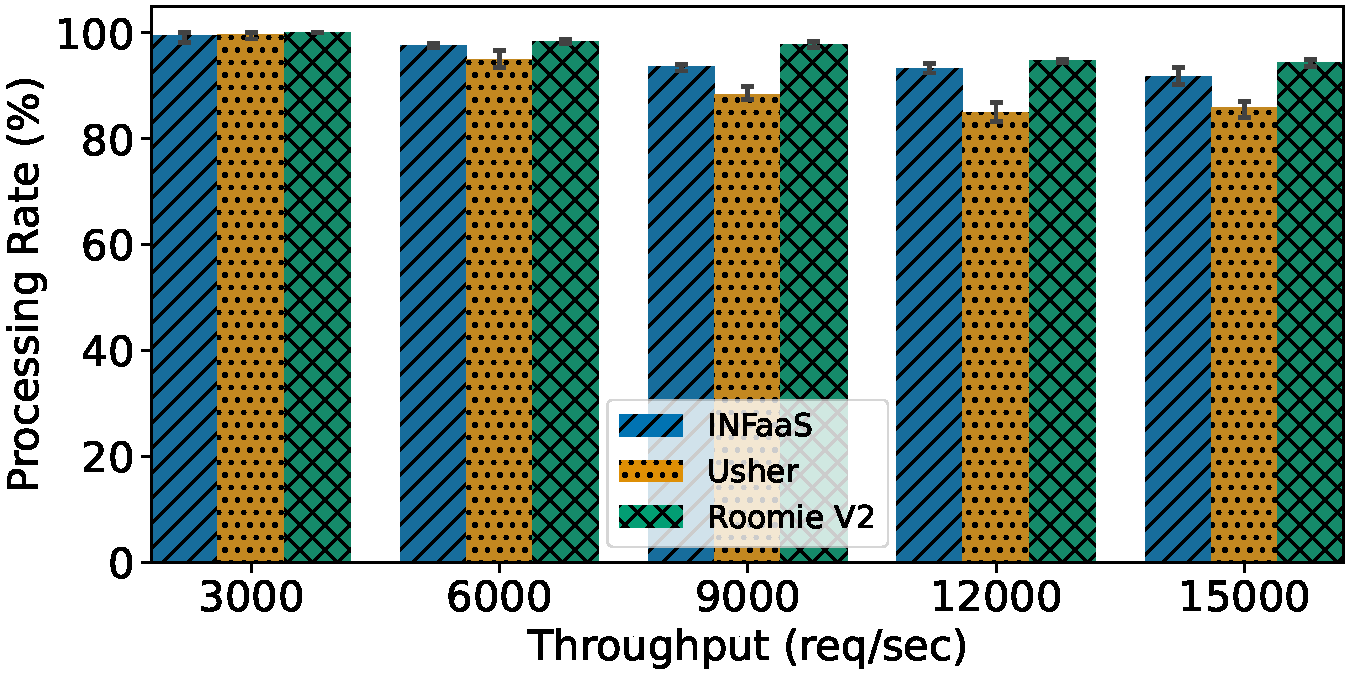
\includegraphics[width=\textwidth]{chapters/roomie/images/NvidiaA100/synthetic-all-models/normalized.pdf}
		\subcaption{Processing rate.}
	\end{subfigure}
	
	\vspace{0.5cm} % Space between the rows
	
	\begin{subfigure}[b]{0.45\textwidth}
		\centering
		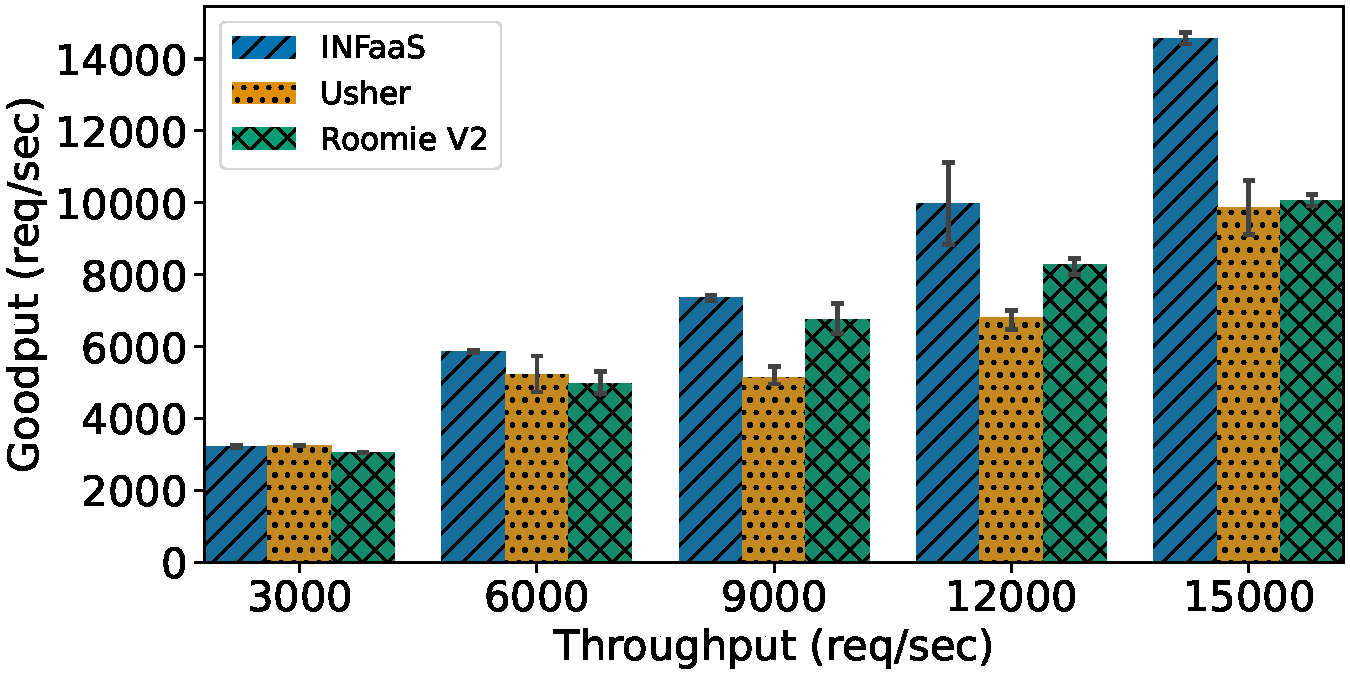
\includegraphics[width=\textwidth]{chapters/roomie/images/NvidiaA100/synthetic-all-models/goodput.pdf}
		\subcaption{Goodput.}
	\end{subfigure}
	\hfill
	\begin{subfigure}[b]{0.45\textwidth}
		\centering
		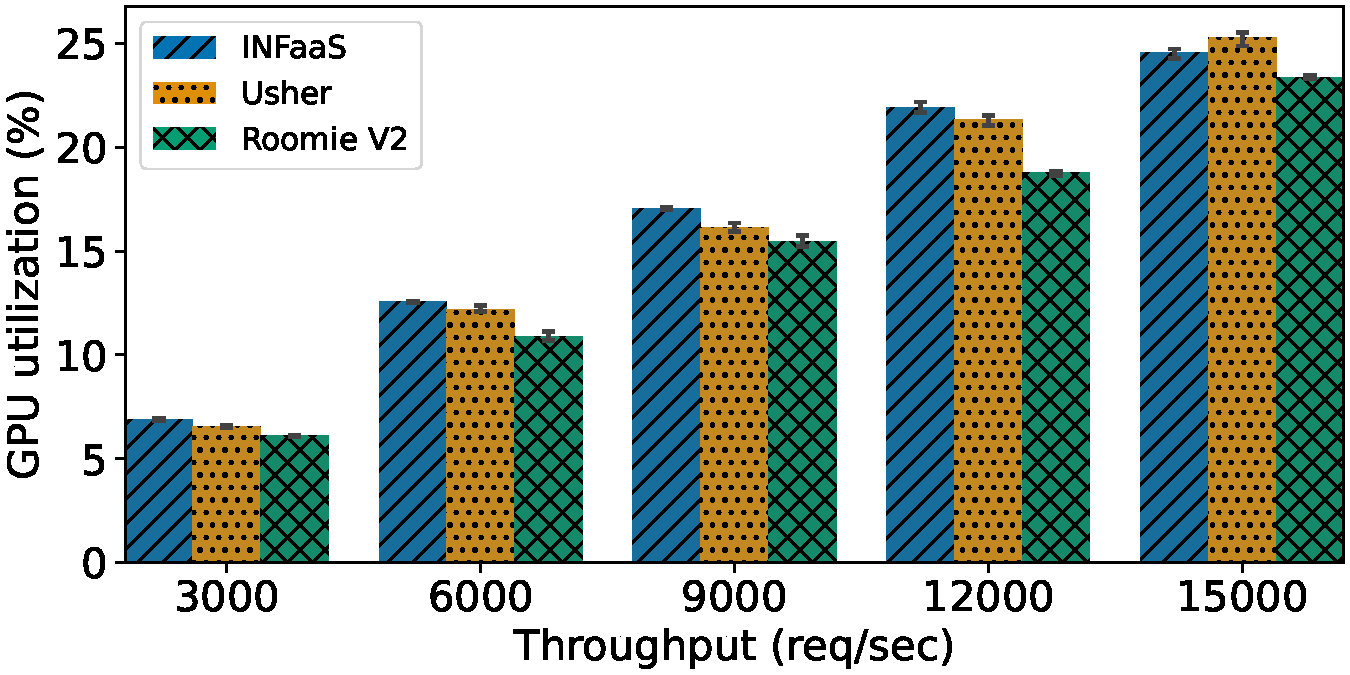
\includegraphics[width=\textwidth]{chapters/roomie/images/NvidiaA100/synthetic-all-models/gpu_utilization.pdf}
		\subcaption{\acrshort{gpu} utilization.}
	\end{subfigure}
	\caption{In cloud-based evaluation using synthetic workloads,~\roomie{} yields 9.2× faster response time and higher processing rate, confirming its deployment efficiency in controlled stress scenarios.}
	\label{fig:NvidiaA100/synthetic-all-models}
	\vspace{-3mm}
\end{figure}


\Cref{fig:NvidiaA100/synthetic-all-models/response-time} illustrates the results of the evaluation conducted with a synthetic dataset designed to emulate diverse and controlled workload scenarios.\\
The performance trends observed with the synthetic dataset closely mirrored those seen with the Twitter data.~\roomie{} consistently outperformed other deployment strategies, achieving a 9.2× reduction in response time and superior throughput and processing rates. These gains are attributed to~\roomie's intelligent model deployment and colocation strategy, which minimizes interference and maximizes resource efficiency.

Overall, across both datasets,~\roomie{} demonstrated robust performance under varying workload conditions. It consistently achieved lower response times—up to 17× faster, and higher processing rate than competing approaches, validating its effectiveness in cloud-based \acrshort{gpu} environments.



\subsection{Performance Evaluation on Edge Devices Using Jetson Xavier \acrshort{gpu}s}

To further validate our approach, we conducted a second set of experiments using a cluster of 12 Jetson Xavier \acrshort{gpu}s, representative of resource-constrained edge computing environments. As in the cloud-based evaluation, we deployed 12 models (from~\Cref{tab:dnn-models}) and tested performance using Twitter data and synthetic data, gradually increasing the workload intensity.

\paragraph{Evaluation on twitter dataset.}

\begin{figure}[h!]
	\centering
	\begin{subfigure}[b]{0.45\textwidth}
		\centering
		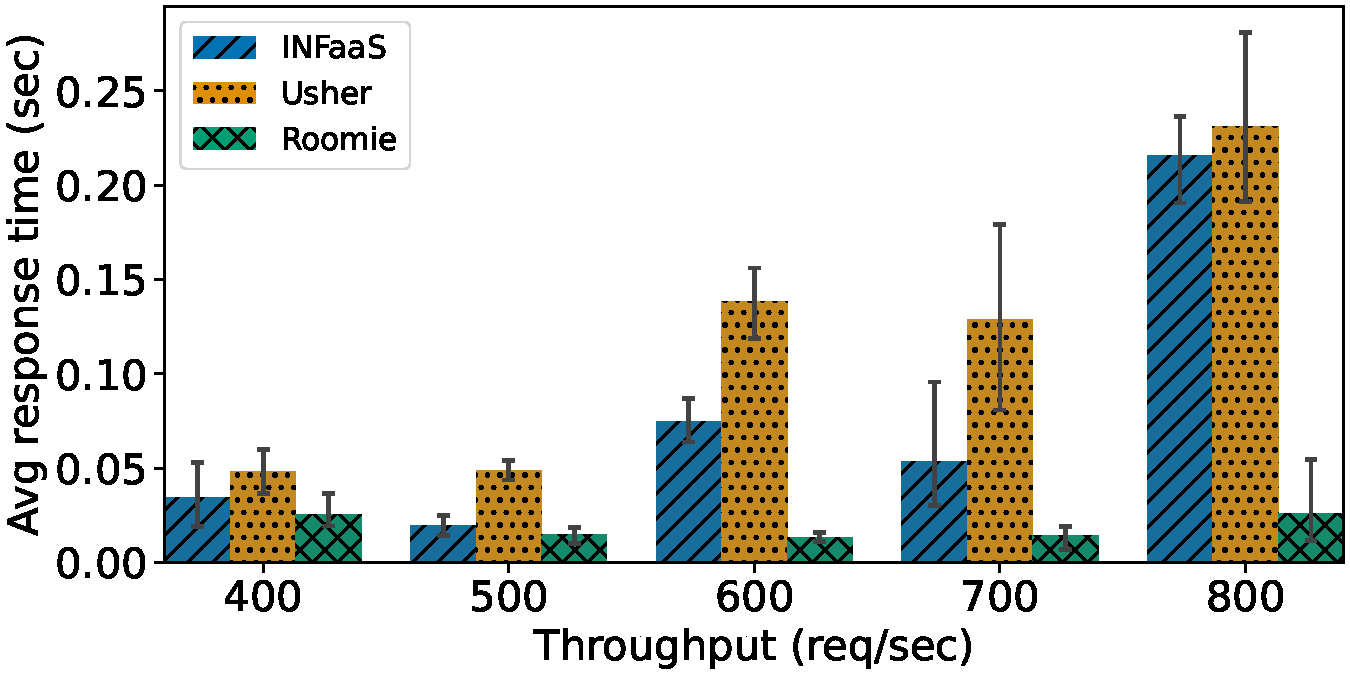
\includegraphics[width=\textwidth]{chapters/roomie/images/JetsonNano/twitter-all-models/response_time.pdf}
		\subcaption{Response time.}
	\end{subfigure}
	\hfill
	\begin{subfigure}[b]{0.45\textwidth}
		\centering
		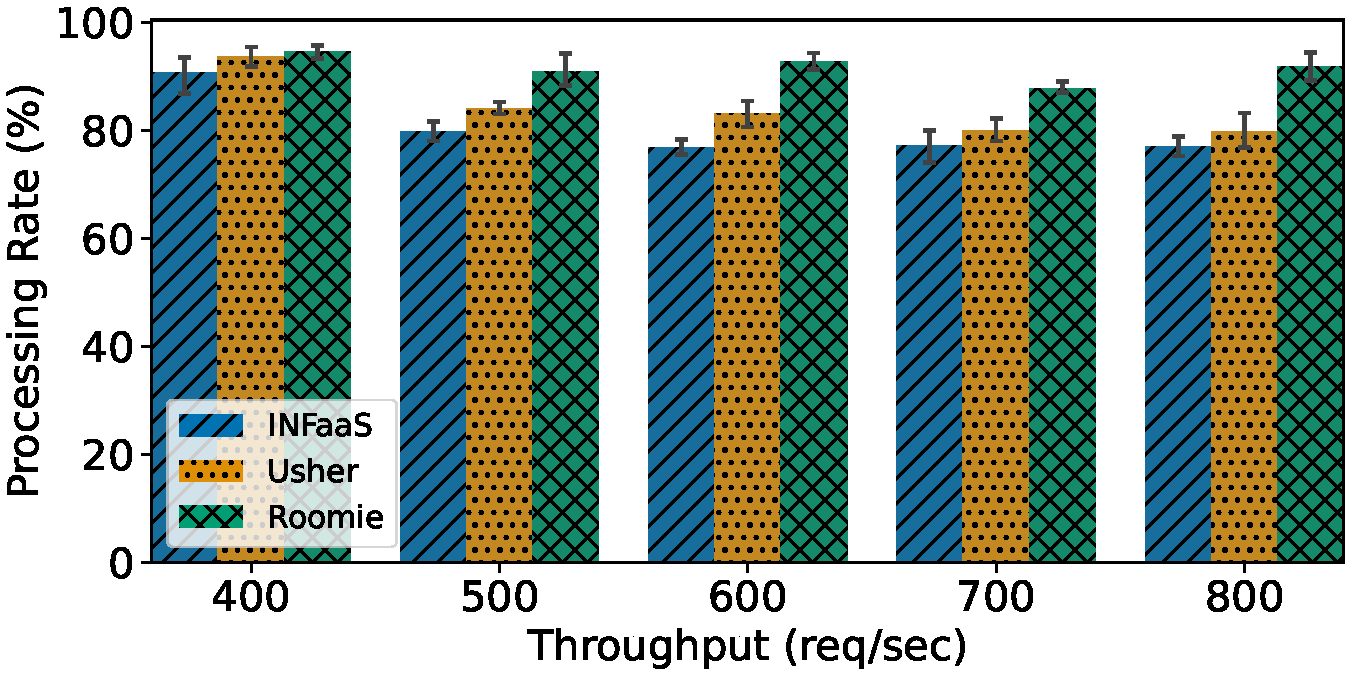
\includegraphics[width=\textwidth]{chapters/roomie/images/JetsonNano/twitter-all-models/normalized.pdf}
		\subcaption{Processing rate.}
	\end{subfigure}
	
	\vspace{0.5cm} % Space between the rows
	
	\begin{subfigure}[b]{0.45\textwidth}
		\centering
		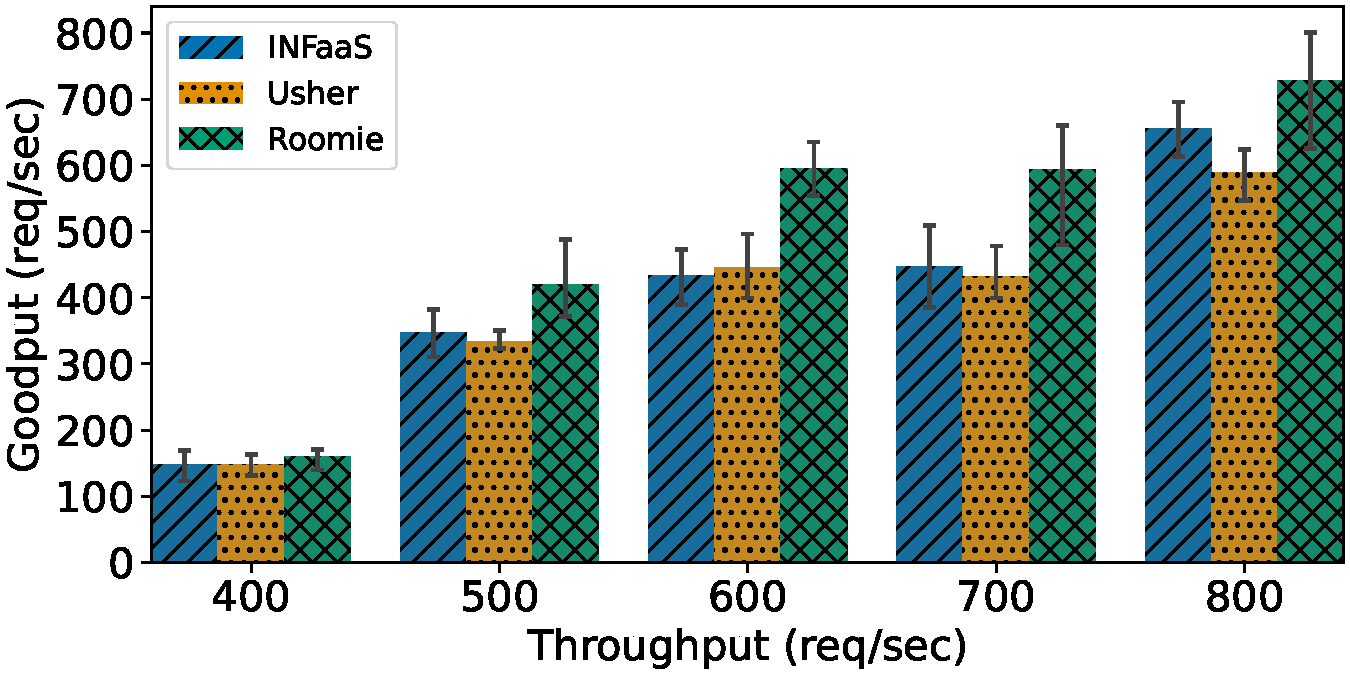
\includegraphics[width=\textwidth]{chapters/roomie/images/JetsonNano/twitter-all-models/goodput.pdf}
		\subcaption{Goodput.}
	\end{subfigure}
	\hfill
	\begin{subfigure}[b]{0.45\textwidth}
		\centering
		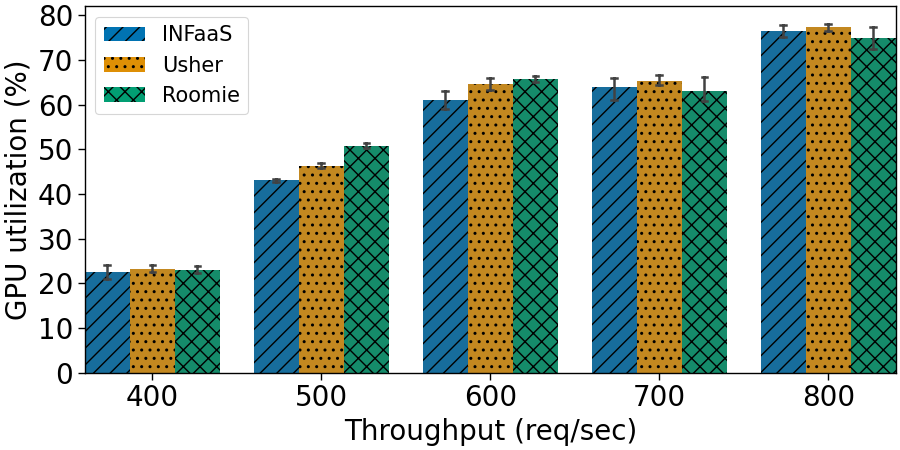
\includegraphics[width=\textwidth]{chapters/roomie/images/JetsonNano/twitter-all-models/gpu_utilization.png}
		\subcaption{\acrshort{gpu} utilization.}
	\end{subfigure}
	\caption{Edge-based evaluation on the Twitter dataset shows~\roomie{} delivering 8.3× lower latency and superior throughput on Jetson Xavier \acrshort{gpu}s, validating its proactive colocation strategy under constrained resources.}
	\label{fig:JetsonNano/twitter-all-models}
	\vspace{-3mm}
\end{figure}

The~\Cref{fig:JetsonNano/twitter-all-models} presents the results obtained with the Twitter dataset on Jetson Xavier devices. While Usher and INFaaS exhibited similar throughput levels, INFaaS achieved lower latency, whereas Usher maintained a higher processing rate.~\roomie, nevertheless, significantly outperformed both, achieving an 8.3× reduction in latency compared to INFaaS under high workload conditions. It also delivered superior throughput and processing rates due to its proactive colocation strategy.

Edge environments impose more severe constraints on model deployment due to limited computing resources and reduced scalability. In this context,~\roomie's colocation strategy offers a significant advantage, effectively balancing resource allocation and minimizing performance degradation. As workload intensity increases, \acrshort{gpu} utilization increases accordingly, reaching levels significantly higher than those seen in cloud-based configurations. This underscores the critical importance of intelligent colocation policies in edge scenarios, where resource efficiency has a direct impact on system responsiveness and throughput.

\paragraph{Evaluation on synthetic dataset.}

\begin{figure}[h!]
	\centering
	\begin{subfigure}[b]{0.45\textwidth}
		\centering
		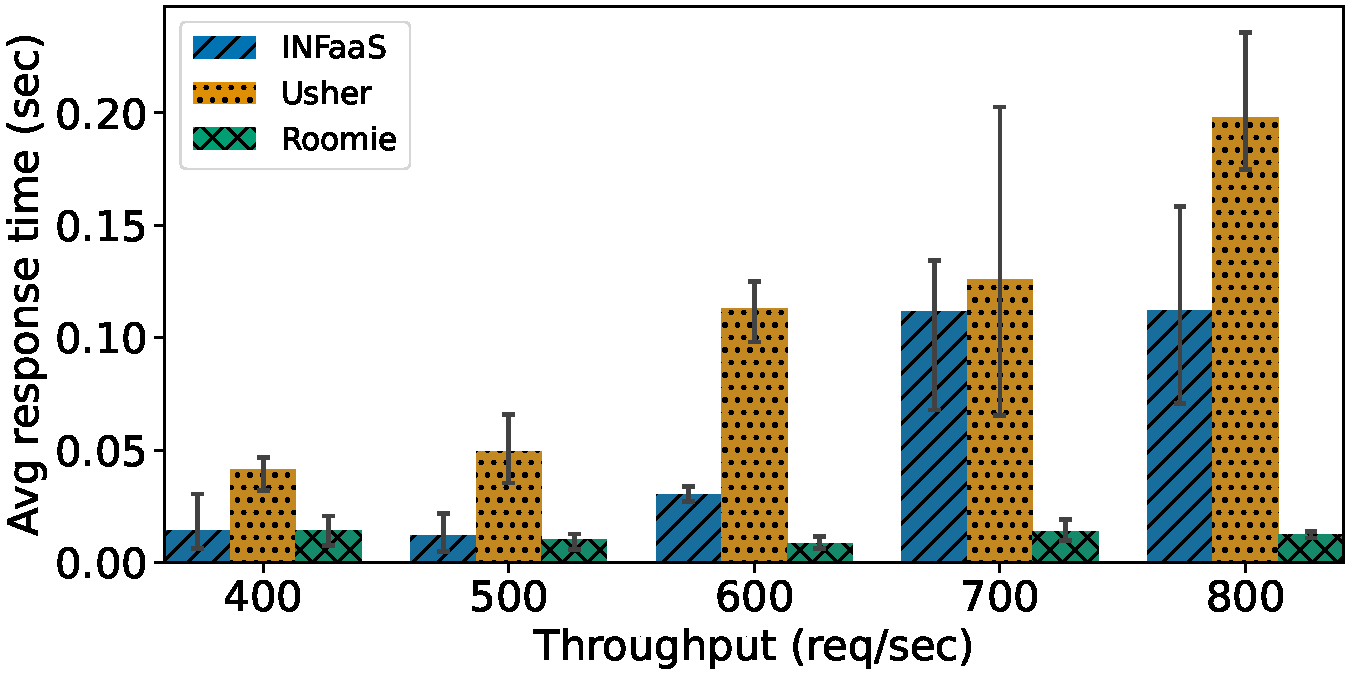
\includegraphics[width=\textwidth]{chapters/roomie/images/JetsonNano/synthetic-all-models/response_time.pdf}
		\subcaption{Response time.}
	\end{subfigure}
	\hfill
	\begin{subfigure}[b]{0.45\textwidth}
		\centering
		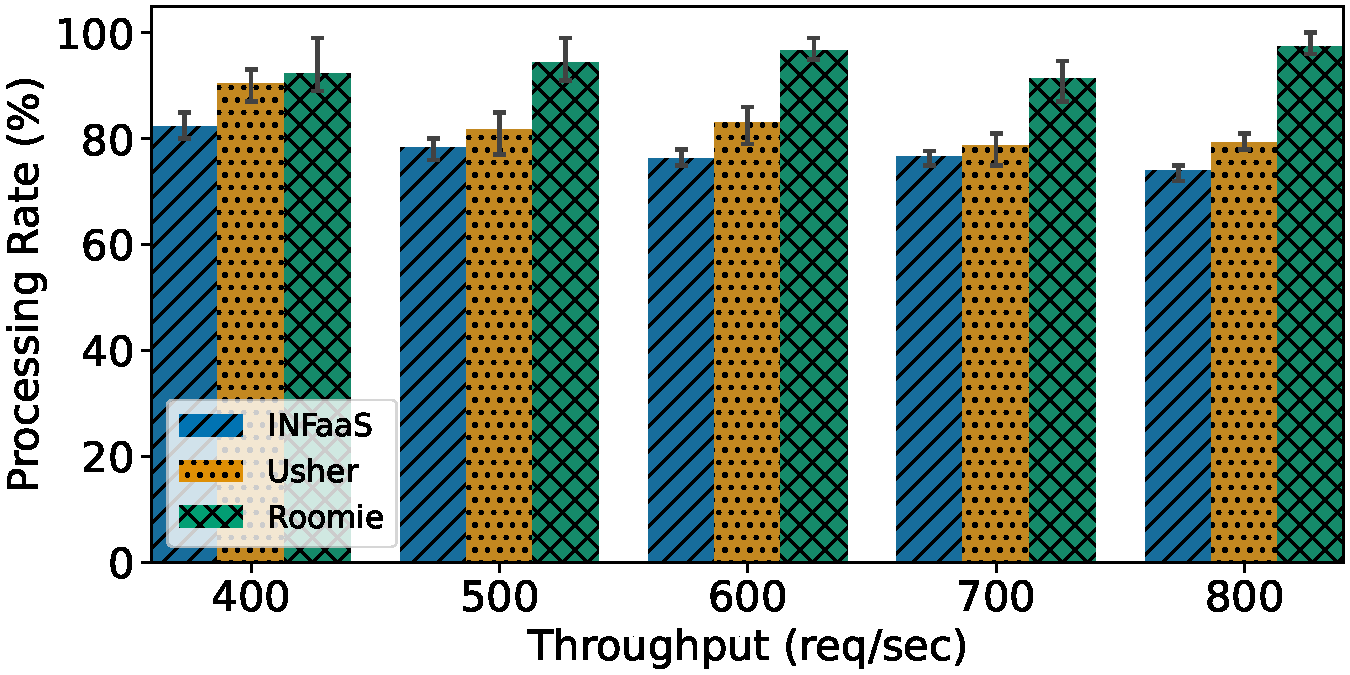
\includegraphics[width=\textwidth]{chapters/roomie/images/JetsonNano/synthetic-all-models/normalized.pdf}
		\subcaption{Processing rate.}
	\end{subfigure}
	
	\vspace{0.5cm} % Space between the rows
	
	\begin{subfigure}[b]{0.45\textwidth}
		\centering
		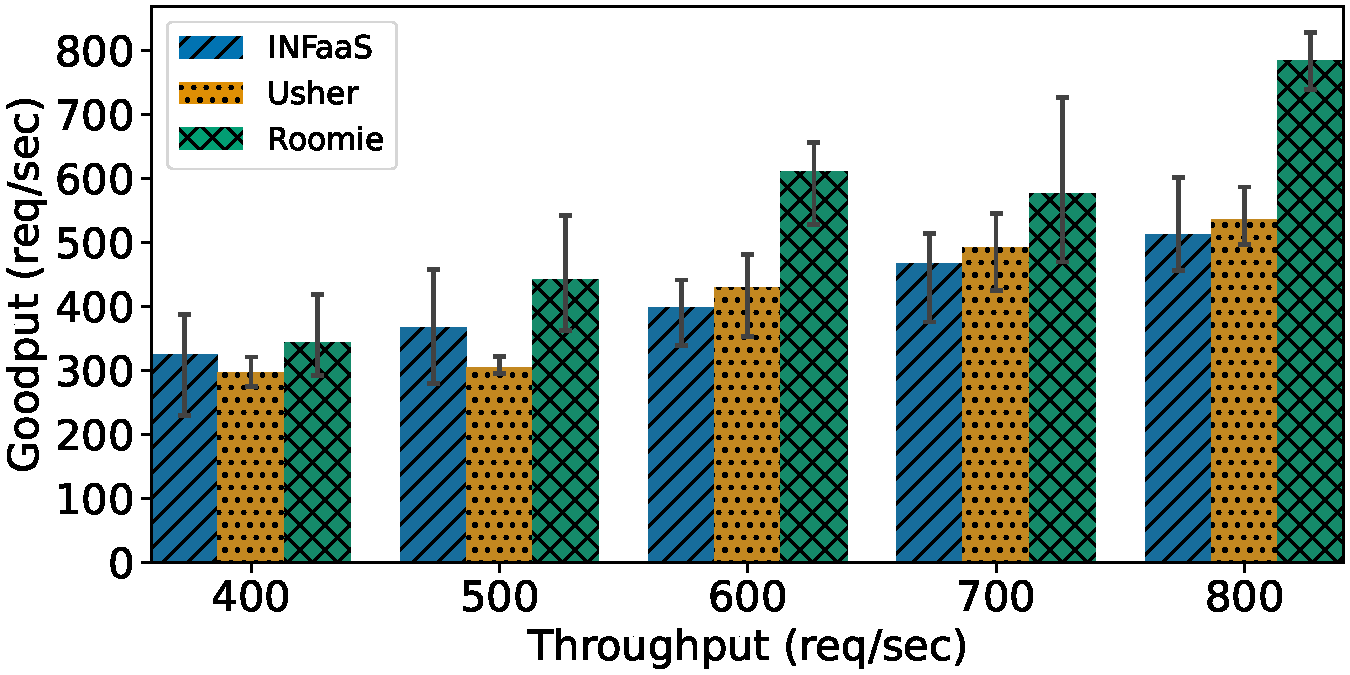
\includegraphics[width=\textwidth]{chapters/roomie/images/JetsonNano/synthetic-all-models/goodput.pdf}
		\subcaption{Goodput.}
	\end{subfigure}
	\hfill
	\begin{subfigure}[b]{0.45\textwidth}
		\centering
		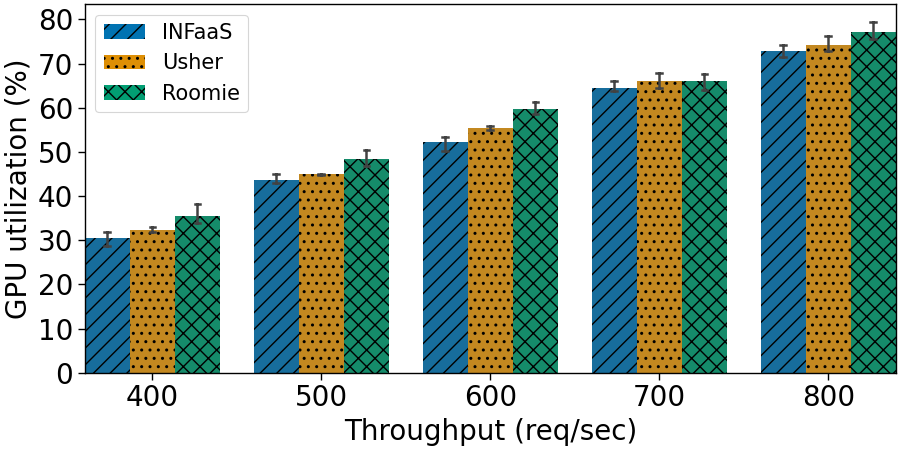
\includegraphics[width=\textwidth]{chapters/roomie/images/JetsonNano/synthetic-all-models/gpu_utilization.png}
		\subcaption{\acrshort{gpu} utilization.}
	\end{subfigure}
	\caption{Under synthetic edge evaluation,~\roomie{} sustains 9× faster response time and 1.5× higher throughput, demonstrating robust performance in resource-limited environments.}
	\label{fig:JetsonNano/synthetic-all-models}
	\vspace{-3mm}
\end{figure}

The synthetic dataset evaluation on Jetson Xavier \acrshort{gpu}s yielded consistent results with those observed on the Twitter dataset. The results are shown in~\Cref{fig:JetsonNano/synthetic-all-models}.~\roomie{} again demonstrated superior performance, achieving a 9× reduction in response time and a 1.3× increase in processing rate. Throughput was also 1.5× higher than competing approaches.

These findings confirm that~\roomie{} is the most effective \acrshort{dnn} deployment strategy in edge computing contexts where colocation is necessary and resources are limited. Its ability to maintain low latency and high throughput under constrained conditions makes it a compelling solution for real-time inference workloads.


\subsection{Evaluating~\roomie{} Deployment Accuracy Against Optimal Strategies}

\begin{figure}[t!]
	\centering
	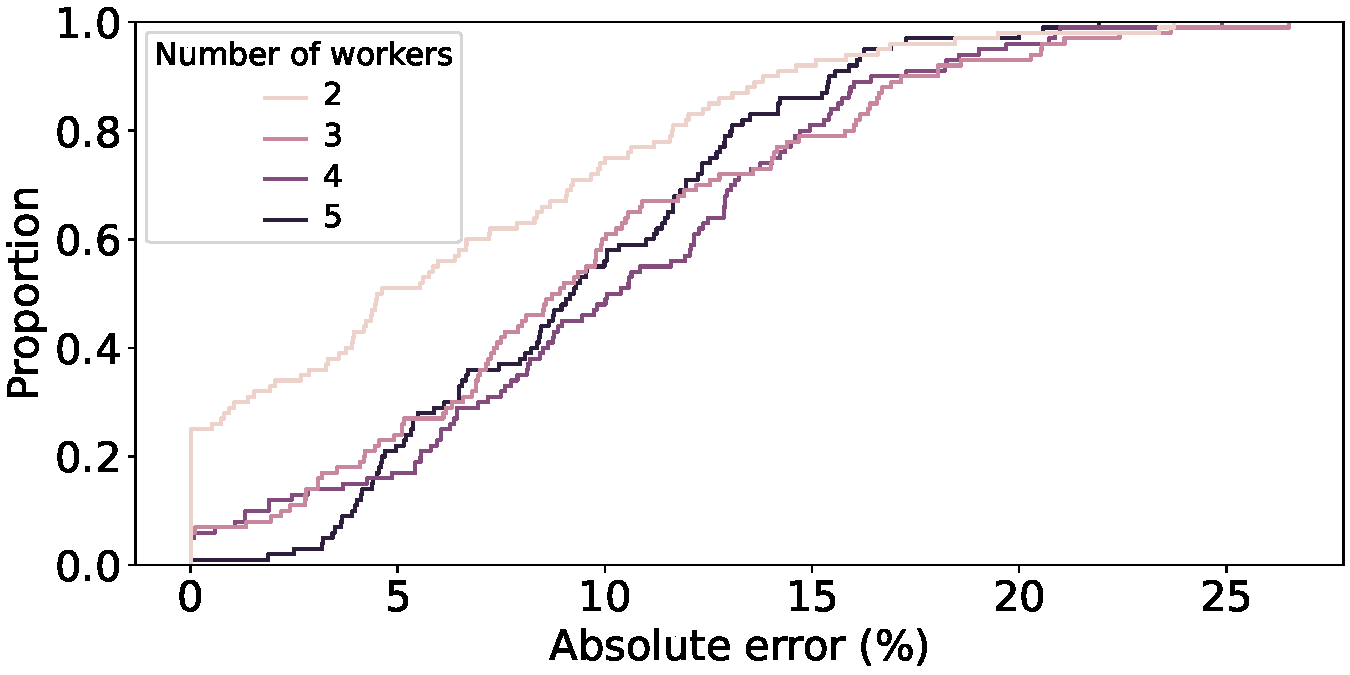
\includegraphics[width=\textwidth]{chapters/roomie/images/performance_gap_per_worker.pdf}
	\caption{Empirical CDF of~\roomie's performance gap relative to the optimal deployment strategy.}
	\label{fig:performance_gap}
\end{figure}

This section investigates the efficacy of~\roomie{} for the deployment of \acrshort{dnn}s across a varying number of workers, specifically between two and five. For each configuration, the quantity of \acrshort{dnn}s to be deployed was randomly selected from a range of two to three times the number of workers, guided by predefined options outlined in~\Cref{tab:dnn-models}. More than 100 randomized evaluations were conducted to ensure comprehensive coverage of deployment scenarios. In each evaluation, all feasible deployment permutations were thoroughly assessed to determine the configuration that resulted in the minimal average performance drop, defined as the optimal baseline. Subsequently, \roomie{} approach was applied to the same scenarios, and the absolute error between \roomie{} and optimal deployments was calculated. The cumulative distribution function (CDF) in~\Cref{fig:performance_gap} summarizes the accuracy of~\roomie{} deployment strategy for deep neural networks (\acrshort{dnn}s).

The first key observation lies in the low-error range. With two workers, 25\% of deployments fall below 0.4\% error, indicating that~\roomie{} often achieves near-optimal results in simple configurations. This sharply contrasts with higher concurrency levels, where the lower quartile rises to over 5\% for three or more workers. This shift reflects the increasing difficulty of estimating performance under competitive conditions, where profiling tools such as Nsight-Compute introduce overhead that distorts kernel execution metrics central to the modeling process.\\
The second key value is the central tendency. The median error climbs from 4\% with two workers to 10\% with four, before slightly receding with five. This peak coincides with the most pronounced modeling challenges, where pairwise colocation and reduced configuration space, used to accelerate convergence, begin to weaken. As concurrency increases,~\roomie{} must account for overlapping execution schedules and interleaved kernels, which obscure the relative timing of model completions and complicate inference behavior.\\
Third, the highest observed errors across configurations do not follow a consistent upward or downward trend, but instead fluctuate with concurrency. It rises from 13\% with two workers to 17\% with three, then drops slightly to 16\% with four and further to 15\% with five. This pattern suggests that while~\roomie{} faces its greatest challenges in intermediate configurations, it regains robustness as the system becomes more distributed. The added flexibility at higher concurrency levels appears to mitigate some of the estimation noise introduced by profiling and architectural interference.

Overall, the analysis demonstrates that~\roomie{} performs reliably under low concurrency and remains competitive even as complexity increases. Its ability to maintain bounded error across a wide range of deployment scenarios is particularly notable given the inherent challenges of performance estimation in \acrshort{gpu} environments. Profiling remains indispensable for capturing fine-grained kernel behavior, despite its overhead and distortion effects.~\roomie's design, grounded in practical strategies such as pairwise colocation and reduced configuration space, proves effective in navigating these constraints. While intermediate concurrency levels expose the limits of current modeling techniques, the overall performance remains within acceptable bounds, validating~\roomie{} as a scalable and interference-aware solution for multi-model deployment.